\documentclass[11pt]{article}
\usepackage[letterpaper,margin=0.9in]{geometry}
\usepackage[hidelinks]{hyperref}
\usepackage{enumitem}
\usepackage{titlesec}
\usepackage{tabularx}
\usepackage{graphicx}

\setlist[itemize]{leftmargin=1.2em,itemsep=3pt,topsep=3pt}
\titleformat{\section}{\large\bfseries}{}{0em}{}[\titlerule]

\newcommand{\entry}[4]{
  \noindent\begin{tabularx}{\textwidth}{@{}Xr@{}}
    \textbf{#1} & #2 \\
    \textit{#3} & \textit{#4}
  \end{tabularx}\vspace{2pt}
}

\begin{document}

\noindent\begin{minipage}[t]{0.76\textwidth}
\vspace{0pt}
{\LARGE \textbf{Piter Z. Garcia Bautista}}\\[4pt]
Rochester, NY \textbar\ +1 (646) 288-3300 \textbar\ \href{mailto:pzg8794@rit.edu}{pzg8794@rit.edu}\\
\href{https://linkedin.com/in/garciapiterz}{linkedin.com/in/garciapiterz} \textbar\
\href{https://github.com/pzg8794}{github.com/pzg8794} \textbar\
\href{https://garciapiterz.com}{garciapiterz.com}
\end{minipage}%
\hfill\begin{minipage}[t]{0.20\textwidth}
\vspace{0pt}
\raggedleft
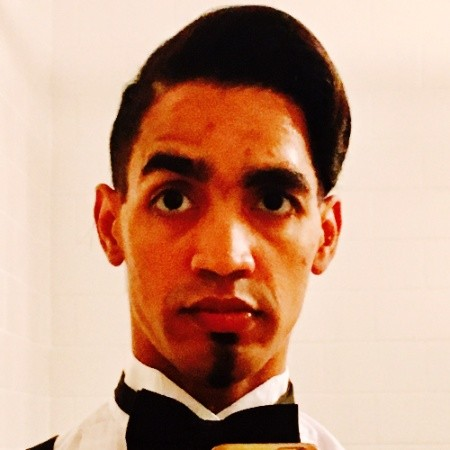
\includegraphics[width=\linewidth]{profile_pic}
\end{minipage}
\vspace{6pt}

\section{Research Profile}
Graduate researcher focused on machine learning for diagnostics and decision support under noisy, heterogeneous, and partially observed data. Background includes an M.S. in Computer Science, current M.S. work in Data Science, industry healthcare AI experience, and computational biology training. Current work emphasizes reproducibility, robust evaluation, fairness-aware analysis, and translational relevance to clinical settings.

\section{Research Interests}
Machine learning for precision medicine and diagnostics; robust learning under missing or uncertain context; fairness-aware and trustworthy AI for high-stakes decision support; reproducible computational evaluation systems.

\section{Education}
\entry{Rochester Institute of Technology}{Expected Aug 2026}{Master of Science, Data Science --- GPA 3.9}{Rochester, NY}
\begin{itemize}
  \item Relevant coursework: Bioinformatics Algorithms, Data-Driven Knowledge Discovery, Neural Networks, Applied Statistics, Software Engineering for Data Science.
\end{itemize}

\entry{Rochester Institute of Technology}{2015}{Master of Science, Computer Science --- GPA 3.2}{Rochester, NY}
\begin{itemize}
  \item Concentrations: Artificial Intelligence, Big Data Analytics, Computer Graphics.
\end{itemize}

\entry{University of Rochester, Warner School of Education}{In progress}{Graduate study, Teaching Computer Science K--12 (M.S. track) --- GPA 4.0}{Rochester, NY}
\begin{itemize}
  \item NSF Robert Noyce Scholar; Advanced Certificate in Leadership in Disability and Inclusive Practices.
\end{itemize}

\entry{Farmingdale State College}{2012}{Bachelor of Science, Computer Engineering Technology --- GPA 3.3}{Farmingdale, NY}
\begin{itemize}
  \item Foundations in computer hardware, embedded systems, and engineering design; early technical training for computational problem-solving.
\end{itemize}

\section{Research and Professional Experience}
\entry{Rochester Institute of Technology, Software Engineering Department}{Fall 2025 -- Present}{Graduate Assistant, Quantum and AI Research}{Rochester, NY}
\begin{itemize}
  \item Build reproducible machine learning evaluation pipelines across local, Colab, and GCP environments with structured logging and validation.
  \item Develop experimental bandit and decision-making systems for uncertain, heterogeneous settings, with emphasis on reliability and traceability.
  \item Produce manuscript-ready technical analyses and research artifacts for faculty-led projects.
\end{itemize}

\entry{Rochester Institute of Technology}{2026}{Computational Biology Research Projects (BIO614 and BIO550)}{Rochester, NY}
\begin{itemize}
  \item Led substantial computational work in BIO614, including formal manuscript development in the project \textit{BIO614-FinalProjectProposal} (Overleaf), emphasizing algorithm implementation, structured evaluation, and scientific reporting.
  \item Complemented BIO614 with BIO550 RNA-seq and differential-expression analysis, including reproducible preprocessing, quality-control validation, and biological interpretation.
\end{itemize}

\entry{VEDADATA Inc.}{Sep 2022 -- Aug 2024}{Data Solutions Engineer}{New York, NY}
\begin{itemize}
  \item Designed scalable Python and pandas workflows for ingestion, validation, preprocessing, and analytics operations.
  \item Strengthened production data reliability through structured quality checks and statistical diagnostics.
\end{itemize}

\entry{VIOME Inc.}{Jan 2021 -- Sep 2022}{AI Data Solutions Engineer}{New York, NY}
\begin{itemize}
  \item Developed healthcare-oriented machine learning workflows for preprocessing, feature engineering, model experimentation, and evaluation.
  \item Supported reproducible analytics workflows in AWS-based environments for predictive health applications.
\end{itemize}

\section{Selected Technical Writing}
\begin{itemize}
  \item \textit{Fairness-Aware Bandits for Network Routing in Quantum and Clinical Settings} (DSCI601 project proposal, manuscript-style report).
  \item \textit{Designing Equitable AI Systems for Diagnostics} (IDAI700 Research Portfolio) --- ethical AI framework for trustworthy diagnostic tools for patients from marginalized communities.
  \item \textit{BIO614-FinalProjectProposal} (Overleaf) and companion BIO550 computational biology analyses on RNA structure and RNA-seq workflows, with reproducible diagnostics-oriented interpretation.
  \item \textit{Equitable Bioinformatics: Enhancing Diagnostic Decision-Making through RNA and Biomarker Data} (ISTE-780 Project Report) --- systematic fairness assessment of ML-driven diagnostic algorithms, with reproducible SHAP-based bias detection and statistical significance testing.
  \item \textit{Predicting Hospital Readmission Rates: A Multi-Method ML Analysis} (DSCI-633 Project Report) --- predictive modeling for clinical risk stratification using ensemble and regularized regression methods.
\end{itemize}

\section{Technical Competencies}
\textbf{Programming:} Python, R, Java, C++, C\#, SQL, MATLAB, JavaScript, Bash\\
\textbf{Machine Learning:} PyTorch, TensorFlow, scikit-learn, XGBoost, model evaluation, uncertainty-aware analysis, fairness-aware ML\\
\textbf{Data and Statistics:} pandas, NumPy, SciPy, statistical modeling, reproducible benchmarking\\
\textbf{Research Tooling:} Git/GitHub, Linux, Docker, LaTeX, AWS, GCP

\section{Selected Fit for KTH Single-Cell Position}
\begin{itemize}
  \item Combined computational biology evidence from BIO614 and BIO550, including manuscript-style technical writing and RNA-seq differential-expression analysis.
  \item Strong Python-based machine learning and reproducibility background for robust method development on high-dimensional, heterogeneous biomedical data.
  \item Clear research motivation for AI and machine learning methods that improve interpretability and reliability in single-cell cancer-data analysis.
\end{itemize}

\end{document}